%--
%  Vistas: está sería la parte principal del TP. Acá irían los diagramas y los
%  escenarios representativos de uso. No necesariamente tiene que ser una gran
%  sección, sino que pueden partirla por funcionalidades y a su vez por tipo de
%  vista o de la forma que crean más pertinente. Esta sección NO DEBE SER una
%  simple seguidilla de figuras sueltas. Debe estar acompañada de tantas
%  explicaciones como sean necesarias para que se aprecie un hilo conductor.
%--
\section{Vistas}

  %--
%-- Diagrama de Contexto
%--
\subsection{Diagrama de Contexto}

%--
%-- Agentes
%--
\subsubsection{Agentes}

\begin{enumerate}
  \item Depósito
  \item Cliente
  \item Sucursal
  \item Sistema
  \item Logística
  \item Departamento de stock 
  \item Agente de Cobro
  \item Administrador
  \item Sistema de Correo Electrónico
  \item Financiera\footnote{Ejemplo: VERAZ}
  \item Correo Argentino
\end{enumerate}
\clearpage

%--
%-- Listado de Fenómenos
%--
\subsubsection{Listado de Fenómenos}
\begin{enumerate}
 \item Configuración y uso por parte del Administrador
  \begin{enumerate}
   \item El Administrador ingresa credenciales en el Sistema
   \item El Administrador define el umbral de redituabilidad en el Sistema
   \item El Administrador consulta estadísticas en el Sistema
  \end{enumerate}

 \item Registro presencial cliente
  \begin{enumerate}
      \item El Cliente se traslada a la Sucursal
      \item El Cliente presenta la documentación en la Sucursal
      \item El Cliente presenta la factura asociada al domicilio en la Sucursal
      \item El Cliente presenta datos de tarjeta en la Sucursal
      \item La Sucursal presenta datos de tarjeta del cliente al Agente de Cobro
      \item El Agente de Cobro verifica la tarjeta de crédito del Cliente
      \item La Sucursal verifica datos personales y de domicilio del Cliente
      \item La Sucursal carga datos del cliente en el Sistema
  \end{enumerate}
  
 \item Registro online cliente
  \begin{enumerate}
    \item El Cliente presenta datos de identificación personal y de domicilio al Sistema
    \item El Cliente presenta datos de pago al Sistema
    \item El Sistema valida domicilio con el Correo Argentino
    \item La Financiera evalúa estado financiero del Cliente
    \item El Agente de Cobro valida datos de pago del Cliente
    \item El Sistema añade al Cliente
  \end{enumerate}
  
 \item Registro pedido
  \begin{enumerate}
    \item El Cliente ingresa credenciales en el Sistema
    \item El Sistema muestra stock disponible al Cliente
    \item El Sistema muestra recomendaciones al Cliente
    \item El Cliente selecciona mercadería en el Sistema
  \end{enumerate}
 
 \item Acuerdo de fecha
  \begin{enumerate}
    \item Logística le calcula el costo de envío al domicilio al Sistema
    \item Si el cliente no recibi\'o alg\'un pedido: 
      \begin{enumerate}
      \item El Sistema bloquea contraentrega al Cliente
      \item El Sistema ofrece pago de multa para salvarlo
      \end{enumerate}
    \item El Sistema contabiliza ingresos producidos por compras del Cliente
    \item El Sistema evalúa ingreso generado por influencia social del Cliente
    \item El Sistema informa métodos de pago disponibles al Cliente
    \item EL Cliente elige forma de pago en el Sistema
    \item Si la forma de pago es online: 
    \begin{enumerate}
      \item El Cliente paga el pedido al Agente de Cobro
      \item El Agente de cobro confirma el pago al Sistema
      \item El Sistema confirma la recepción del pago al Cliente
    \end{enumerate}
  \end{enumerate}
  
 \item Modificaci\'on de pedido
  \begin{enumerate}
    \item El Cliente modifica un pedido no cerrado en el Sistema
    \item El Sistema le dá un crédito al Cliente si este quita mercadería paga
  \end{enumerate}

 \item Preparación y entrega
  \begin{enumerate}
    \item El Cliente confirma el pedido al Sistema
    \item El Sistema avisa al Depósito que prepare el pedido 
    \item El Depósito informa egreso de mercadería al Departamento de stock
    \item El Depósito avisa al Sistema que el pedido está cerrado
    \item El Depósito entrega mercadería a Logística
    \item Si forma de pago es contraentrega: 
    \begin{enumerate}
      \item Cliente paga el pedido a Logística
    \end{enumerate}
    \item Logística entrega el pedido al Cliente
    \item El Sistema actualiza positivamente el perfil del Cliente
  \end{enumerate}

 \item Entrega fallida
  \begin{enumerate}
    \item El Cliente no recibe pedido a Logística
    \item El Sistema reintegra el dinero al Cliente si este no lo recibe
    \item El Sistema añade una no-recepción al historial de recepciones del Cliente
    \item Logística devuelve el stock al Depósito
    \item El Sistema de Correo electrónico ofrece rehacer el pedido Cliente
  \end{enumerate}

 \item Reposicion stock sucursal
  \begin{enumerate}
    \item La Sucursal avisa cuando falta stock al Sistema
    \item El Sistema avisa falta de stock en sucursal al Depósito
    \item El Depósito arma pedido y entrega el stock a Logística
    \item El Sistema disminuye stock en el Depósito
    \item Logística entrega stock a la Sucursal
  \end{enumerate}

 \item Reposicion stock deposito
  \begin{enumerate}
    \item El Departamento de stock modifica los límite m\'inimos de stock estipulado para cada producto en el Sistema
    \item El Sistema avisa que hay faltante de producto al Departamento de stock
    \item El Departamento de stock encarga reposición de stock del depósito a Logística
    \item Logística repone stock al Depósito
  \end{enumerate}

 \item Cierre de sesi\'on
  \begin{enumerate}
    \item Cliente cierra sesión en el Sistema
    \item Administrador	cierra sesión en el Sistema
  \end{enumerate}
\end{enumerate}
\clearpage

%--
%-- Acciones Básicas
%--
\subsubsection{Diagrama de Contexto}

\begin{figure}[H]
  \begin{center}
  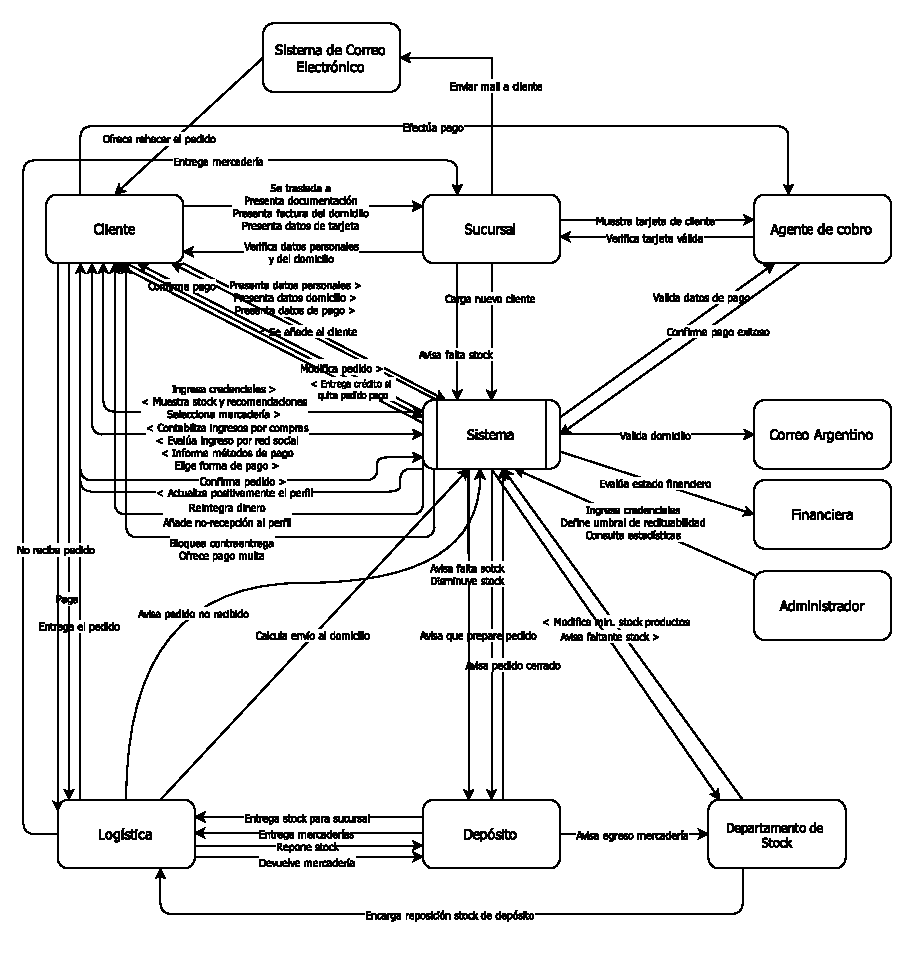
\includegraphics[height=0.65\textheight,angle=90]{images/contexto.pdf}
  \end{center}
\end{figure}


  %--
%-- Modelo de Objetivos
%--
\clearpage
\subsection{Modelo de Objetivos}

\subsubsection{Diagrama de Objetivos}
\fixme[Insertar el diagrama (no entra en una página)]

\newpage
\subsubsection{Objetivo blando: Registro del cliente}
\begin{figure}[H]
  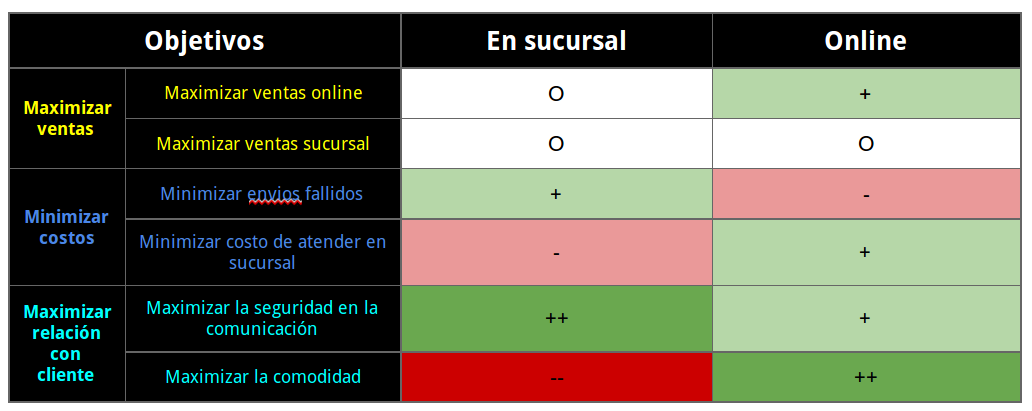
\includegraphics[width=\linewidth]{images/objetivo-blando-registro-cliente.png}
\end{figure}

\paragraph{Ventas}

La opción de registro online es evidentemente más simple y accesible, lo que
ocasionaría que más clientes opten por registrarse y comprar online, sobre todo
aquellos clientes que no acostumbran a comprar normalmente en ese supermercado
(ya que esto no impactaría tanto en los clientes habituales). De lo anterior, se
deduce que la opción de registro online impactaría positivamente en el objetivo
de maximizar las ventas online.

\paragraph{Costos}

Al obligar a los clientes a registrarse presencialmente en una sucursal,
exigiendoles la documentación correspondiente (por ejemplo, dni, un impuesto,
una factura de servicio) que acredite su domicilio y su identidad, se estaría
obteniendo una verificación confiable de los mismos, lo que repercute en una
minimización de los envíos fallidos ocasionados por personas que presentan datos
falsos, o sin ser esta su intención, cometen errores al escribir los datos. El
registro online, por el contrario, aumenta la posibilidad de que sucedan esos
inconvenientes, lo que impactaría negativamente en la minimización de los envíos
fallidos.

\paragraph{Relación con cliente}

\subparagraph{Maximizar la seguridad en la comunicación:}

Al registrar los datos del cliente en la sucursal, en persona, se presume que la
transmisión de los datos del cliente es siempre más segura que si se lo hace
online. De todos modos, según lo solicitado por el CEO, la comunicación se
establecería por un canal seguro, así que el riesgo de robo de información por
medio de una escucha de red se encuentra notablemente suprimido. Desde esa
perspectiva, ambos canales de comunicación tienen un nivel de confiabilidad
similar.

Por otro lado, mediante el canal de registro online, una persona podría llegar a
realizar un registro fraudulento, suplantando la identidad de otra persona,
escudada en el anonimato que ofrece internet, mientras que presencialmente es
mucho más difícil realizar este tipo de prácticas, de lo que concluimos que, si
bien ambos canales son seguros, la vía presencial resulta bastante más
confiable.

\subparagraph{Maximizar la comodidad:}

Obligar al cliente a realizar el registro presencialmente, suponiendo además que
este deba recolectar y presentar toda la documentación pertinente, le puede
llegar a resultar molesto e incómodo. En el peor caso el cliente tendría que
juntar y fotocopiar toda la documentación exigida, dirigirse a una sucursal en
horario laboral, no necesariamente cerca de su domicilio, esperar a ser
atendido, completar algún tipo de formulario, entregar la documentación, y
esperar a que le informen de algún modo que su usuario fue dado de alta.
Mediante el registro online, en cambio, el cliente podrá ingresar al website
desde la comodidad de su casa, en cualquier horario, e ingresar sus datos.
Inmediatamente, entonces, el cliente tendría la posibilidad de realizar una
compra.

\newpage
\subsubsection{Objetivo blando: Ranking del cliente}
\begin{figure}[H]
  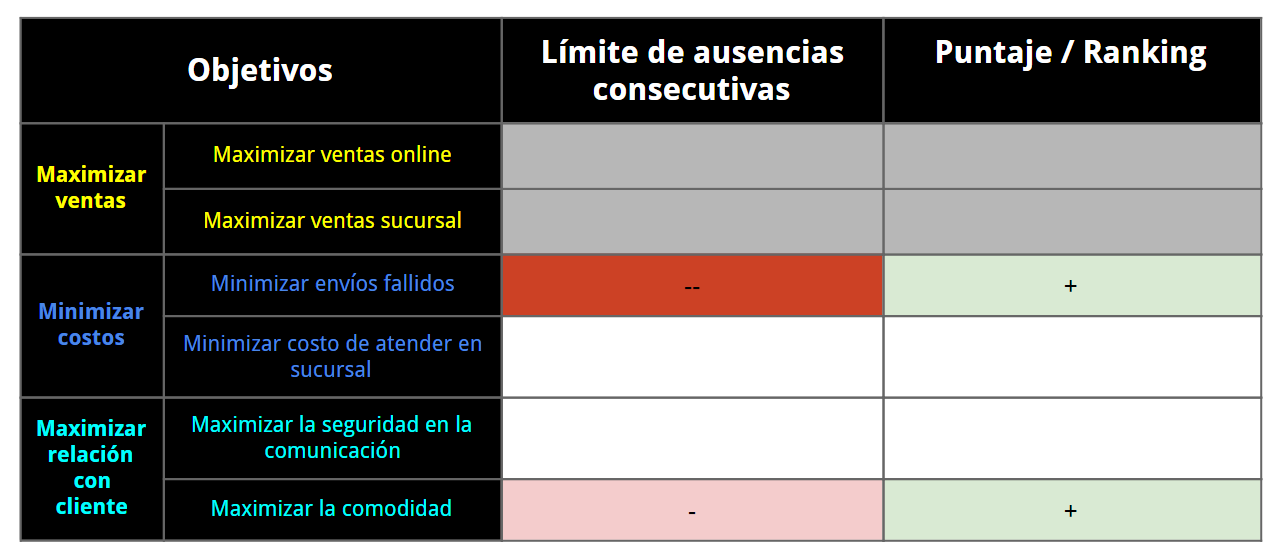
\includegraphics[width=\linewidth]{images/objetivo-blando-ranking-cliente.png}
\end{figure}

\fixme[Agregar completar tabla y agregar texto justificando los puntajes]

  %--
%-- Escenarios de uso
%--  
\newpage
\subsection{Escenarios representativos de uso}

%-- Escenario 1
\subsubsection{A: Registro online}

\textbf{\emph{Alice}} no es cliente habitual de la cadena mesporciento, ya que
le queda lejos de su casa como para ir caminando. Tras enterarse de la nueva
posibilidad de comprar online, se conecta al sitio web www.mesporciento.com a
través de su computadora, y registra un nuevo usuario
``\texttt{alice\_gatita93}'', ingresando para ello sus \textbf{datos
personales}, tales como nombre, domicilio, teléfono, email, y una
\textbf{contraseña segura}. El sitio verifica que los datos ingresados son
correctos, y luego le envía un mail de confirmación con un vínculo en el que
\textbf{\emph{Alice}} presiona para validar su cuenta. \textbf{\emph{Alice}}
entonces reingresa al sitio, utilizando ahora su nuevo usuario.

%-- Escenario 2
\subsubsection{B: Registro presencial con sistema de reputación}

\textbf{\emph{Bob}} es cliente habitual de la cadena mesporciento, y aprovecha
una de sus rutinarias compras para registrar su usuario en su sitio web. Para
ello, se encargó previamente de juntar la documentación requerida para el
registro: el documento de identidad, y una acreditación de domicilio, en
particular lleva la última factura de luz. Luego de las compras, le pregunta a
la cajera en dónde debe registrarse, y le indican que se dirija a la sección de
informes.

En la sección de informes no hay nadie, por lo que \textbf{\emph{Bob}} debe
esperar unos 10 minutos hasta que aparezca la encargada. Esta le pide la
documentación, y la verifica mientras le entrega a \textbf{\emph{Bob}} un
cuestionario de datos personales para que lo complete. Luego,
\textbf{\emph{Bob}} le entrega el cuestionario, y la empleada verifica que los
datos del cuestionario y la documentación coincidan. Entonces, le saca
fotocopias a la documentación y al cuestionario. Le entrega la fotocopia del
cuestionario a \textbf{\emph{Bob}}, mientras que la fotocopia de la
documentación es archivada junto con el cuestionario en un sobre de papel
madera, que a su vez es apilado junto a muchos otros sobres de aspecto similar.
Finalmente, le informa a \textbf{\emph{Bob}} que se le avisará por mail en
cuanto el registro se encuentre completo, y allí mismo le brindarán las
instrucciones para acceder al sitio.

Luego de dos semanas, \textbf{\emph{Bob}} recibe un email de parte del remitente
felicitaciones@mesporciento.com, y asunto <<Bienvenido a una nueva forma de
comprar>>, en el que se le informa que ya se encuentra habilitado su usuario
``\texttt{marley\_b420}''

%-- Escenario 3
\subsubsection{C: Pago online}

\textbf{\emph{Charlie}} se conecta a la web de mesporciento desde su tablet, con
su usuario ``\texttt{je\_suis\_moi}'', dispuesto a iniciar su compra de
productos semanal, de forma online. Para ello, revisa el listado de productos, y
agrega a su \textbf{carrito virtual} los que necesita. Una vez que el carrito
contiene todos los productos que desea, presiona el botón \texttt{``FINALIZAR
COMPRA''}, el cual lo dirige a la pantalla de cierre de pedido. En esta
pantalla, se le informa del costo total de la compra, y se le ofrecen opciones
de fechas y horarios posibles de entrega, de entre las que
\textbf{\emph{Charlie}} elige el Miércoles de la semana que viene, por la
mañana, ya que sabe que en ese horario va a estar en su casa.

Luego, en la siguiente pantalla, elige la opción de Pago Online, y el sitio le
solicita que elija un método de pago de entre las distintas opciones
disponibles. Ya que \textbf{\emph{Charlie}} confía mucho en el sistema
\texttt{PayPal}, lo elige, tras lo cual se abre una ventana externa que redirige
al sitio de PayPal, en que tras ingresar su usuario y su clave se le solicita
confirmar el valor de la compra. Luego de que esta ventana se cierra, el sitio
le muestra una animación muy jocosa de un tigre mirando un reloj, mientras
debajo se puede leer la frase \texttt{``Por favor, espere, estamos validando el
pago...''}. Tras unos segundos, el tigre comienza a bailar, el mensaje se
desvanece, y lo reemplaza un nuevo mensaje \texttt{``Su pago se encuentra
confirmado. Le hemos enviado un mail con la información de su pedido. Gracias
por confiar en nosotros. En unos instantes, será redirigido a la página
principal.''}.

%-- Escenario 4
\subsubsection{D: Pago contrareembolso}

\textbf{\emph{Dave}} tiene un problema de adicción al casino. Normalmente, con
la ayuda de sus amigos y familiares, lo controla sin mayores inconvenientes.
Pero hace 1 semana tuvo un viaje laboral, y en el último día, libre para todos
los empleados, no resistió la tentación de jugar una o dos tiradas de ruleta,
con el efectivo que llevaba encima. Tuvo la mala suerte de que le fue
relativamente bien, ganó ambas jugadas lo que le hizo cuadruplicar su efectivo.
Envalentonado por su repentino y misterioso golpe de suerte, se dirigió a la
casilla de venta de fichas, y gastó todo el dinero de su cuenta bancaria en
fichas. También compró fichas con su tarjeta de crédito, en un pago, hasta
alcanzar el límite. Compró en total 450 fichas, y volvió a dirigirse a la
ruleta. Su plan inicial era realizar una paciente Martingala, pero un rayo
cósmico atravesó su mente momentos antes de colocar la apuesta, y supo entonces
que debía elegir el número 7. Claro, porque este era el séptimo día del viaje
laboral, y había tenido mucha suerte, por lo que el siete era un buen número.
Claramente, \textbf{\emph{Dave}} perdió todo su dinero, y no solo eso, sino que
se endeudó gravemente, saturando el límite de su tarjeta de crédito.

Al volver a su casa, le cuenta lo sucedido a su tío, pidiéndole que no le cuente
a nadie, y este le presta dinero ``hasta que logre salir de la situación''. Como
no tiene tiempo de ir al supermercado, ya que debe hacer horas extras para pagar
sus deudas, aprovecha el sistema de compras online de mesporciento para encargar
las provisiones de la semana durante la noche. Se autentica en el sitio con su
usuario, ``\texttt{lucky\_guy\_00}'', elige los productos indispensables para el
resto del mes, y pacta una fecha de entrega para el día siguiente. Al momento de
elegir la opción de pago, advierte que no puede realizar un pago online, ya que
la tarjeta se encuentra saturada, por lo que opta por elegir la opción de pago
contrareembolso.

Al otro día, temprano, suena el timbre, y recibe el pedido, el cual paga en
efectivo, y les deja una modesta propina a los muchachos para que carguen las
bolsas hasta la cocina de su casa.

%-- Escenario 5
\subsubsection{E: Entrega correcta}

El Martes 13 de Abril \textbf{\emph{Erin}} realizó un pedido de torta de
cumpleaños, cotillón y un regalo grandioso para ser entregado el Martes
siguiente, en conmemoración del 50-cumpleaños de su tía. Aprovecha la
posibilidad para elegir que su pedido sea entregado en la casa de su tía, y no
en su domicilio. Para ello, intenta modificar el domicilio de su usuario
``\texttt{ireland\_green}'', pero el sistema no se lo permite. Entonces, como
\textbf{\emph{Erin}} es muy inteligente, crea un nuevo usuario
``\texttt{tia\_50}'', especial para esta ocasión, el cual completa con los datos
de su tía. Por comodidad, además, lo paga en línea, con una tarjeta de crédito
(la suya, no la de su tía), ya que por costumbre familiar está prohibido hablar
de dinero durante el cumpleaños de una tía, y quiere evitar malos momentos
durante el episodio festivo.

Llegado el día, están todos festejando, ya con algunas copitas encima, cuando la
tía grita a \textbf{\emph{Erin}}: <<¿y la torta? ¿y los juguetitos que me habías
prometido?>>. En ese instante, justamente, suena el timbre, y resultan ser los
empleados de mesporciento. \textbf{\emph{Erin}} les abre la puerta y les indica
dónde dejar la mercadería. Les dice que no puede darles propina por una
costumbre familiar, tras lo cual los empleados regresan a su camión,
apesumbrados.

%-- Escenario 6
\subsubsection{F: Ausente durante entrega}

\textbf{\emph{Frank}} es una persona muy olvidadiza. Tanto es así, que durante
la mañana de hoy, fue hasta el banco a cobrar un cheque, para terminar dándose
cuenta que no lo había llevado. No fue sino hasta la mañana del día siguiente,
al leer su email, que se enteró que, durante su ausencia en el banco, había
recibido una visita del supermercado Mes\%, al cual había justamente encargado
una compra el día anterior. Utilizando un vínculo provisto dentro del mismo
mensaje, programó la visita para ese mismo día, al mediodía, y luego se ató un
piolín en el dedo corazón para recordarlo. Entonces miró un poco de televisión,
y tras terminar el programa, cuando se dispuso a cambiar de canal, se dio cuenta
que su dedo, el del piolín obviamente, estaba totalmente ennegrecido y arrugado.
Peor aún, a pesar de desatarlo, este había perdido la sensibilidad, y no
recuperaba su rosadito color habitual. \textbf{\emph{Frank}} se asustó tanto,
que corrió raudo hasta la calle, y tomó un taxi hasta el hospital más cercano,
sin advertir que estaba en pijama, y que este no dejaba nada a la imaginación.
En el hospital, les explicó que, por razones que no podemos repetir, para él era
muy importante este dedo, y que no podía perderlo. Entonces le dieron una bata
para que pueda poner sobre el pijama y proteger la sensibilidad del resto de los
pacientes, y le realizaron estrambóticos procedimientos médicos. Luego de un par
de horas \textbf{\emph{Frank}} pudo recuperar el funcionamiento habitual de su
dedo. Cuando el médico le preguntó que por qué se le había puesto así el dedo,
\textbf{\emph{Frank}} le explicó que se había atado algo. Tras lo cual el médico
hizo una obvia segunda pregunta, lo cual provocó algo similar a un click en
algún recóndito lugar del cerebro de \textbf{\emph{Frank}}, seguido de una
catarata de imágenes mentales, la mayoría de ellas relacionadas al supermercado
Mes\%. Entonces, repentinamente, se levantó, corrió hasta la puerta del
hospital, y tomó un taxi nuevamente hasta su casa. Al llegar, abrió su mail,
para enterarse de que nuevamente había perdido la entrega. Se le informaba,
además, de que su usuario ``\texttt{f\_estein}'' había perdido la posibilidad de
realizar compras contrareembolso, hasta pagar una multa de \$100, lo cual
ciertamente lo puso de muy mal humor.

\subsubsection{G: Cancelación de pedido}

\textbf{\emph{Gabriel}} había hecho un pedido el lunes a la mañana. A la tarde
descubre mejores precios en los chinos de la vuelta, y decide cancelar la compra
para hacerla en ese lugar que le resulta más económico (haciendo las cuentas,
llega a la conclusión de que con la diferencia podía comprar un videojuego para
sus hijos). Entonces, vuelve rápido de los chinos a su casa, y entusiasmado
chequea que aún pueda hacer la cancelación. Para ello ingresa al sitio
\texttt{www.mesporciento.com} con su cuenta ``\texttt{gabi\_25x8}'' poniendo sus
datos, seleccionando el pedido vigente. Selecciona la opción de modificación de
pedido y posteriormente, al comprobar que no está cerrado, lo cancela.

El sistema le confirma la cancelación. Finalmente \textbf{\emph{Gabriel}} vuelve
contento a los chinos a hacer la compra y con lo que le sobra, compra el
videojuego para sus hijos (¡aunque como padre responsable, primero lo juega el
para enseñarle a ellos!).

\subsubsection{H: Modificación de pedido}

En la casa de \textbf{\emph{Helena}} van a festejar la navidad. Unas horas
después de que había hecho un pedido para preparar la cena, surgió que además de
la familia, fueron invitados su amiga \textbf{\emph{Hermenegilda}} con sus hijos
para no pasar la navidad solos debido a que el marido de
\textbf{\emph{Hermenegilda}} y sus parientes aún no regresaron del exterior por
asuntos laborales. Por este motivo, \textbf{\emph{Helena}} decide modificar el
pedido que tenía hecho incrementando la cantidad de productos comprados como por
ejemplo las gaseosas. Para eso entra al sitio \texttt{www.mesporciento.com}
ingresando sus datos, chequea que aún no haya sido cerrado dicho pedido, y al
comprobarlo selecciona la opción de modificarlo. El sistema le confirma la
modificación.

\subsubsection{Administración inteligente de productos de depósitos}

\fixme[El administrador ingresa al sistema, ve estadísticas, 
modifica productos vigentes (abm)]

\subsection{Alarma y reposición por bajo stock en depósitos}
Luego de que una clienta comprara diez pack de gaseosas Coca-Cola, se agotó el stock de dicho producto, por lo que saltó 
la alarma del sistema. El sistema entonces le avisa al Departamento de Stock de forma automática. Un superior del 
Departamento de Stock recibe el aviso y hace los pedidos correspondientes a Logística, quien finalmente se encarga de 
reponer el stock.
% Hay que hablar de que alguien le confirma ls sistema que se hizo la reposicion y no se si tambien de otras cosas.

\fixme[Se agota el stock, salta alarma, sistema avisa a dpto de stock, 
dpto de stock hace pedidos, avisa a logística, y se repone stock]

\subsection{Preparar y cerrar pedido}     %¿En realidad no sería cerrar y preparar?
\textbf{\emph{Bastián}}, un empleado de la sucursal, entra al sitio \texttt{www.mesporciento.com\texttt} y revisa 
los pedidos pendientes. Selecciona el primero que aparece en la lista (están ordenados por prioridad) y lo cierra. Luego 
lo prepara poniendo en una caja los productos encargados.  
% ¿Empleado de la sucursal esta bien?
% ¿Como entra al sitio el empleado Bastián? ¿Igual que los clientes?

\fixme[El sistema avisa a depósito que llegó un pedido,
depósito lo prepara, depósito avisa a sistema que cerró pedido]
